%% Fig. 1 (E1), written by experiments/make_figure.py from results/e1.json (10,000 replicates per size) and Eq. (2)
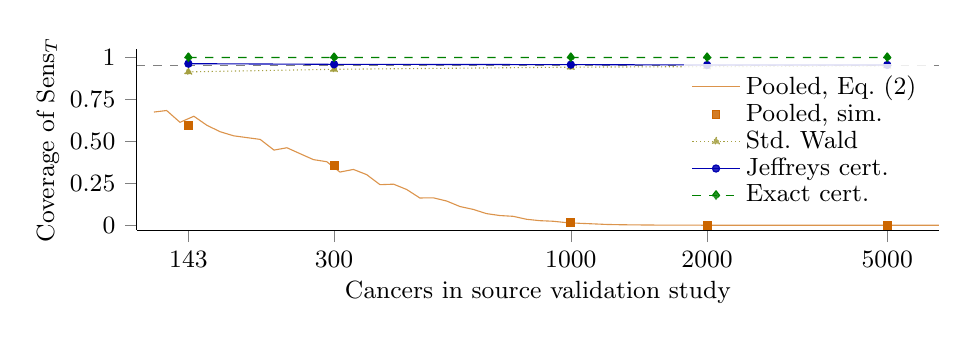
\begin{tikzpicture}
\begin{semilogxaxis}[scale only axis, width=0.84\columnwidth, height=2.3cm,
  xmin=110, xmax=6500, ymin=-0.03, ymax=1.05,
  xtick={143,300,1000,2000,5000}, xticklabels={143,300,1000,2000,5000},
  ytick={0,0.25,0.5,0.75,1}, yticklabels={0,0.25,0.50,0.75,1},
  tick label style={font=\small}, label style={font=\small},
  xlabel={Cancers in source validation study}, ylabel={Coverage of $\mathrm{Sens}_T$},
  ylabel style={yshift=-3pt}, xlabel style={yshift=2pt},
  legend style={font=\small, draw=none, fill=white, fill opacity=0.85, text opacity=1, at={(0.99,0.07)}, anchor=south east, row sep=-2pt},
  legend cell align=left, axis lines*=left, tick align=outside]
\addplot[gray, dashed, thin, forget plot] coordinates {(110,0.95) (6500,0.95)};
\addplot[orange!80!black, thin, opacity=0.7] coordinates {(120,0.6748) (128,0.6840) (137,0.6135) (147,0.6498) (157,0.5963) (168,0.5575) (180,0.5331) (193,0.5220) (206,0.5117) (221,0.4480) (236,0.4619) (253,0.4251) (270,0.3912) (289,0.3786) (309,0.3170) (331,0.3326) (354,0.3018) (379,0.2417) (406,0.2447) (434,0.2129) (464,0.1624) (497,0.1633) (532,0.1441) (569,0.1114) (609,0.0941) (651,0.0692) (697,0.0577) (746,0.0530) (798,0.0355) (854,0.0271) (914,0.0236) (978,0.0154) (1046,0.0114) (1119,0.0081) (1198,0.0046) (1281,0.0030) (1371,0.0020) (1467,0.0013) (1570,0.0007) (1680,0.0004) (1797,0.0002) (1923,0.0001) (2058,0.0000) (2202,0.0000) (2356,0.0000) (2521,0.0000) (2697,0.0000) (2886,0.0000) (3088,0.0000) (3304,0.0000) (3535,0.0000) (3783,0.0000) (4048,0.0000) (4331,0.0000) (4634,0.0000) (4959,0.0000) (5306,0.0000) (5677,0.0000) (6075,0.0000) (6500,0.0000)};
\addlegendentry{Pooled, Eq.~(2)}
\addplot[only marks, mark=square*, mark size=1.4pt, orange!80!black] coordinates {(143,0.5945) (300,0.3559) (1000,0.0144) (2000,0.0000) (5000,0.0000)};
\addlegendentry{Pooled, sim.}
\addplot[densely dotted, mark=triangle*, mark size=1.6pt, yellow!60!black] coordinates {(143,0.9145) (300,0.9297) (1000,0.9425) (2000,0.9456) (5000,0.9500)};
\addlegendentry{Std.\ Wald}
\addplot[mark=*, mark size=1.3pt, blue!70!black] coordinates {(143,0.9633) (300,0.9594) (1000,0.9576) (2000,0.9554) (5000,0.9556)};
\addlegendentry{Jeffreys cert.}
\addplot[dashed, mark=diamond*, mark size=1.7pt, green!50!black] coordinates {(143,1.0000) (300,0.9999) (1000,1.0000) (2000,1.0000) (5000,1.0000)};
\addlegendentry{Exact cert.}
\end{semilogxaxis}
\end{tikzpicture}
